% LaTeX-Vorlage für Versuchsprotokolle
% Autor: Simon May
% Datum: 2017-10-05

% Es gibt die Dokumenttypen scrartcl („Artikel“), scrreprt („Bericht“),
% scrbook („Buch“) und scrlttr2 („Brief“). Diese gehören zum KOMA-Script,
% bieten mehr Optionen als die „Standardklassen“ und sollten besonders für
% deutsche Texte benutzt werden.
% Natürlich gibt es noch weitere Klassen, z.B. beamer für Präsentationen.
\documentclass[
	a4paper,                % Papierformat (DIN A4)
	titlepage=firstiscover, % Separate Titelseite
	captions=tableheading,  % \caption bei Tabellen immer als Überschrift setzen
	toc=bibliography,       % Literaturverzeichnis im Inhaltsverzeichnis aufführen
	toc=listof,             % Abbildungsverzeichnis etc. im Inhaltsverzeichnis aufführen
	oneside,                % Einseitig
	%twoside,               % Zweiseitig
	%twocolumn,             % Zweispaltig
	automark,               % Abschnittstitel automatisch in Kopfzeile einfügen
	12pt,                   % Schriftgröße (beliebige Größen mit „fontsize=Xpt“)
	english, ngerman,       % Sprache für z.B. Babel; ausgewählt: ngerman (letztgenannt)
	%draft=true             % Entwurf-Modus; markiert zu lange und zu kurze Zeilen
]{scrartcl}

% --- Pakete einbinden
% Autor: Simon May
% Datum: 2017-10-04

% --- Pakete einbinden
% --- Pakete erweitern LaTeX um zusätzliche Funktionen.
%     Dies ist ein Satz nützlicher Pakete.

% Silbentrennung etc.; Sprache wird durch Option bei \documentclass festgelegt
\usepackage{babel}
\usepackage{iftex}
\ifLuaTeX
	% Schriftart (Latin Modern)
	\usepackage{fontspec}
	\fontspec{Latin Modern Roman}
\else
	% Verwendung der Zeichentabelle T1 (für Sonderzeichen etc.)
	\usepackage[T1]{fontenc}
	% Legt die Eingabe-Zeichenkodierung fest, z.B. UTF-8
	\usepackage[utf8]{inputenc}
	% Schriftart (Latin Modern)
	\usepackage{lmodern}
	% Zusätzliche Sonderzeichen
	\usepackage{textcomp}
\fi

% Nutzen von +, -, *, / in \setlength u.ä. (z.B. \setlength{\a + 3cm})
\usepackage{calc}
% Wird benötigt, um \ifthenelse zu benutzen
\usepackage{xifthen}
% Optionen für eigene definierte Befehle
\usepackage{xparse}

% Verbessertes Aussehen des Schriftbilds durch kleine Anpassungen
\usepackage{microtype}
% Automatische Formatierung von Daten
\usepackage[useregional]{datetime2}
% Wird für Kopf- und Fußzeile benötigt
\usepackage{scrlayer-scrpage}
% Einfaches Wechseln zwischen unterschiedlichen Zeilenabständen
\usepackage{setspace}
% Optionen für Listen (enumerate, itemize, …)
\usepackage{enumitem}
% Automatische Anführungszeichen
\usepackage{csquotes}
% Zusätzliche Optionen für Tabellen (tabular)
\usepackage{array}

% Mathepaket (intlimits: Grenzen über/unter Integralzeichen)
\usepackage[intlimits]{amsmath}
% Mathe-Symbole, \mathbb etc.
\usepackage{amssymb}
% Weitere Mathebefehle
\usepackage{mathtools}
% „Schöne“ Brüche im Fließtext
\usepackage{xfrac}
% Ermöglicht die Nutzung von \SI{Zahl}{Einheit} u.a.
\usepackage{siunitx}
% Definition von Unicode-Symbolen; Nach [utf8]inputenc laden!
\usepackage{newunicodechar}
% Unicode-Formeln mit pdfLaTeX
% Autor: Simon May
% Datum: 2015-03-04

% Diese Datei ermöglicht es, Mathe-Symbole (z.B. \gamma) direkt als
% Sonderzeichen (d.h. γ) einzugeben

% silence unterdrückt Warnungen; vor hyperref laden
\usepackage{silence}
\WarningFilter[pdflatex-unicode-math]{newunicodechar}{Redefining Unicode character}
\ActivateWarningFilters[pdflatex-unicode-math]

\newunicodechar{†}{\dag}
\newunicodechar{‡}{\ddag}
\newunicodechar{…}{\ldots}
\newunicodechar{⋯}{\cdots}
\newunicodechar{⋮}{\vdots}
\newunicodechar{⋱}{\ddots}
\newunicodechar{⋰}{\iddots}
\newunicodechar{α}{\alpha}
\newunicodechar{β}{\beta}
\newunicodechar{γ}{\gamma}
\newunicodechar{δ}{\delta}
\newunicodechar{ε}{\varepsilon}
\newunicodechar{ϵ}{\epsilon}
\newunicodechar{ζ}{\zeta}
\newunicodechar{η}{\eta}
\newunicodechar{θ}{\theta}
\newunicodechar{ϑ}{\vartheta}
\newunicodechar{ι}{\iota}
\newunicodechar{κ}{\kappa}
\newunicodechar{ϰ}{\varkappa}
\newunicodechar{λ}{\lambda}
\newunicodechar{μ}{\mu}
\newunicodechar{ν}{\nu}
\newunicodechar{ξ}{\xi}
\newunicodechar{ο}{o}
\newunicodechar{π}{\pi}
\newunicodechar{ρ}{\rho}
\newunicodechar{ϱ}{\varrho}
\newunicodechar{σ}{\sigma}
\newunicodechar{τ}{\tau}
\newunicodechar{υ}{\upsilon}
\newunicodechar{φ}{\varphi}
\newunicodechar{ϕ}{\phi}
\newunicodechar{χ}{\chi}
\newunicodechar{ψ}{\psi}
\newunicodechar{ω}{\omega}
\newunicodechar{Α}{\mathrm{A}}
\newunicodechar{Β}{\mathrm{B}}
\newunicodechar{Γ}{\Gamma}
\newunicodechar{Δ}{\Delta}
\newunicodechar{Ε}{\mathrm{E}}
\newunicodechar{Ζ}{\mathrm{Z}}
\newunicodechar{Η}{\mathrm{H}}
\newunicodechar{Θ}{\Theta}
\newunicodechar{Ι}{\mathrm{I}}
\newunicodechar{Κ}{\mathrm{K}}
\newunicodechar{Λ}{\Lambda}
\newunicodechar{Μ}{\mathrm{M}}
\newunicodechar{Ν}{\mathrm{N}}
\newunicodechar{Ξ}{\Xi}
\newunicodechar{Ο}{\mathrm{O}}
\newunicodechar{Π}{\Pi}
\newunicodechar{Ρ}{\mathrm{P}}
\newunicodechar{Σ}{\Sigma}
\newunicodechar{Τ}{\mathrm{T}}
\newunicodechar{Υ}{\Upsilon}
\newunicodechar{Φ}{\Phi}
\newunicodechar{Χ}{\Chi}
\newunicodechar{Ψ}{\Psi}
\newunicodechar{Ω}{\Omega}
\newunicodechar{∑}{\sum}
\newunicodechar{∫}{\int}
\newunicodechar{∬}{\iint}
\newunicodechar{∭}{\iiint}
\newunicodechar{⨌}{\iiiint}
\newunicodechar{∮}{\oint}
\newunicodechar{∯}{\oiint}
\newunicodechar{∰}{\oiiint}
\newunicodechar{∇}{\nabla}
\newunicodechar{∂}{\partial}
\newunicodechar{√}{\sqrt}
\newunicodechar{∈}{\in}
\newunicodechar{∋}{\ni}
\newunicodechar{∉}{\notin}
\newunicodechar{∀}{\forall}
\newunicodechar{∃}{\exists}
\newunicodechar{∄}{\nexists}
\newunicodechar{∴}{\therefore}
\newunicodechar{∵}{\because}
\newunicodechar{〈}{\langle}
\newunicodechar{〉}{\rangle}
\newunicodechar{⌊}{\lfloor}
\newunicodechar{⌋}{\rfloor}
\newunicodechar{⌈}{\lceil}
\newunicodechar{⌉}{\rceil}
\newunicodechar{∼}{\sim}
\newunicodechar{∝}{\propto}
\newunicodechar{∞}{\infty}
\newunicodechar{ℵ}{\aleph}
\newunicodechar{ℏ}{\hbar}
\newunicodechar{℘}{\wp}
\newunicodechar{ℓ}{\ell}
\newunicodechar{∅}{\emptyset}
\newunicodechar{×}{\times}
\newunicodechar{⋅}{\cdot}
\newunicodechar{÷}{\div}
\newunicodechar{⋆}{\star}
\newunicodechar{∘}{\circ}
\newunicodechar{⋄}{\diamond}
\newunicodechar{⊕}{\oplus}
\newunicodechar{⊖}{\ominus}
\newunicodechar{⊗}{\otimes}
\newunicodechar{⊘}{\oslash}
\newunicodechar{⊙}{\odot}
\newunicodechar{±}{\pm}
\newunicodechar{∓}{\mp}
\newunicodechar{≈}{\approx}
\newunicodechar{≡}{\equiv}
\newunicodechar{≠}{\ne}
\newunicodechar{≥}{\ge}
\newunicodechar{≤}{\le}
\newunicodechar{≫}{\gg}
\newunicodechar{≪}{\ll}
\newunicodechar{⊂}{\subset}
\newunicodechar{⊃}{\supset}
\newunicodechar{⊆}{\subseteq}
\newunicodechar{⊇}{\supseteq}
\newunicodechar{⊈}{\nsubseteq}
\newunicodechar{⊉}{\nsupseteq}
\newunicodechar{≔}{\coloneqq}
\newunicodechar{≕}{\eqqcolon}
\newunicodechar{¬}{\neg}
\newunicodechar{∨}{\vee}
\newunicodechar{∧}{\wedge}
\newunicodechar{∪}{\cup}
\newunicodechar{∩}{\cap}
\newunicodechar{⋁}{\bigvee}
\newunicodechar{⋀}{\bigwedge}
\newunicodechar{⋃}{\bigcup}
\newunicodechar{⋂}{\bigcap}
\newunicodechar{⟂}{\perp}
\newunicodechar{∥}{\parallel}
\newunicodechar{∦}{\nparallel}
\newunicodechar{𝚤}{\imath}
\newunicodechar{𝚥}{\jmath}
\newunicodechar{⇔}{\Leftrightarrow}
\newunicodechar{⇕}{\Updownarrow}
\newunicodechar{⇐}{\Leftarrow}
\newunicodechar{⇒}{\Rightarrow}
\newunicodechar{⇑}{\Uparrow}
\newunicodechar{⇓}{\Downarrow}
\newunicodechar{↔}{\leftrightarrow}
\newunicodechar{↕}{\updownarrow}
\newunicodechar{←}{\leftarrow}
\newunicodechar{→}{\rightarrow}
\newunicodechar{↑}{\uparrow}
\newunicodechar{↓}{\downarrow}
\newunicodechar{⟷}{\longleftrightarrow}
\newunicodechar{⟵}{\longleftarrow}
\newunicodechar{⟶}{\longrightarrow}
\newunicodechar{⇇}{\leftleftarrows}
\newunicodechar{⇉}{\rightrightarrows}
\newunicodechar{⇈}{\upuparrows}
\newunicodechar{⇊}{\downdownarrows}
\newunicodechar{⟺}{\Longleftrightarrow}
\newunicodechar{⟸}{\Longleftarrow}
\newunicodechar{⟹}{\Longrightarrow}
\newunicodechar{↦}{\mapsto}
\newunicodechar{↤}{\mapsfrom}
\newunicodechar{⟼}{\longmapsto}
\newunicodechar{⟻}{\longmapsfrom}
\newunicodechar{⟾}{\Longmapsto}
\newunicodechar{⟽}{\Longmapsfrom}
\newunicodechar{↗}{\nearrow}
\newunicodechar{↖}{\nwarrow}
\newunicodechar{↘}{\searrow}
\newunicodechar{↙}{\swarrow}
\newunicodechar{↩}{\hookleftarrow}
\newunicodechar{↪}{\hookrightarrow}
\newunicodechar{↶}{\curvearrowleft}
\newunicodechar{↷}{\curvearrowright}
\newunicodechar{↺}{\circlearrowleft}
\newunicodechar{↻}{\circlearrowright}
\newunicodechar{↫}{\looparrowleft}
\newunicodechar{↬}{\looparrowright}
\newunicodechar{⇋}{\leftrightharpoons}
\newunicodechar{⇌}{\rightleftharpoons}
\newunicodechar{↼}{\leftharpoonup}
\newunicodechar{↽}{\leftharpoondown}
\newunicodechar{⇀}{\rightharpoonup}
\newunicodechar{⇁}{\rightharpoondown}
\newunicodechar{↿}{\upharpoonleft}
\newunicodechar{↾}{\upharpoonright}
\newunicodechar{⇃}{\downharpoonleft}
\newunicodechar{⇂}{\downharpoonright}
\newunicodechar{𝔸}{\mathbb{A}}
\newunicodechar{𝔹}{\mathbb{B}}
\newunicodechar{ℂ}{\mathbb{C}}
\newunicodechar{𝔻}{\mathbb{D}}
\newunicodechar{𝔼}{\mathbb{E}}
\newunicodechar{𝔽}{\mathbb{F}}
\newunicodechar{𝔾}{\mathbb{G}}
\newunicodechar{ℍ}{\mathbb{H}}
\newunicodechar{𝕀}{\mathbb{I}}
\newunicodechar{𝕁}{\mathbb{J}}
\newunicodechar{𝕂}{\mathbb{K}}
\newunicodechar{𝕃}{\mathbb{L}}
\newunicodechar{𝕄}{\mathbb{M}}
\newunicodechar{ℕ}{\mathbb{N}}
\newunicodechar{𝕆}{\mathbb{O}}
\newunicodechar{ℙ}{\mathbb{P}}
\newunicodechar{ℚ}{\mathbb{Q}}
\newunicodechar{ℝ}{\mathbb{R}}
\newunicodechar{𝕊}{\mathbb{S}}
\newunicodechar{𝕋}{\mathbb{T}}
\newunicodechar{𝕌}{\mathbb{U}}
\newunicodechar{𝕍}{\mathbb{V}}
\newunicodechar{𝕎}{\mathbb{W}}
\newunicodechar{𝕏}{\mathbb{X}}
\newunicodechar{𝕐}{\mathbb{Y}}
\newunicodechar{ℤ}{\mathbb{Z}}
\newunicodechar{𝒜}{\mathcal{A}}
\newunicodechar{ℬ}{\mathcal{B}}
\newunicodechar{𝒞}{\mathcal{C}}
\newunicodechar{𝒟}{\mathcal{D}}
\newunicodechar{ℰ}{\mathcal{E}}
\newunicodechar{ℱ}{\mathcal{F}}
\newunicodechar{𝒢}{\mathcal{G}}
\newunicodechar{ℋ}{\mathcal{H}}
\newunicodechar{ℐ}{\mathcal{I}}
\newunicodechar{𝒥}{\mathcal{J}}
\newunicodechar{𝒦}{\mathcal{K}}
\newunicodechar{ℒ}{\mathcal{L}}
\newunicodechar{ℳ}{\mathcal{M}}
\newunicodechar{𝒩}{\mathcal{N}}
\newunicodechar{𝒪}{\mathcal{O}}
\newunicodechar{𝒫}{\mathcal{P}}
\newunicodechar{𝒬}{\mathcal{Q}}
\newunicodechar{ℛ}{\mathcal{R}}
\newunicodechar{𝒮}{\mathcal{S}}
\newunicodechar{𝒯}{\mathcal{T}}
\newunicodechar{𝒰}{\mathcal{U}}
\newunicodechar{𝒱}{\mathcal{V}}
\newunicodechar{𝒲}{\mathcal{W}}
\newunicodechar{𝒳}{\mathcal{X}}
\newunicodechar{𝒴}{\mathcal{Y}}
\newunicodechar{𝒵}{\mathcal{Z}}
\newunicodechar{𝕬}{\mathfrak{A}}
\newunicodechar{𝕭}{\mathfrak{B}}
\newunicodechar{𝕮}{\mathfrak{C}}
\newunicodechar{𝕯}{\mathfrak{D}}
\newunicodechar{𝕰}{\mathfrak{E}}
\newunicodechar{𝕱}{\mathfrak{F}}
\newunicodechar{𝕲}{\mathfrak{G}}
\newunicodechar{𝕳}{\mathfrak{H}}
\newunicodechar{𝕴}{\mathfrak{I}}
\newunicodechar{𝕵}{\mathfrak{J}}
\newunicodechar{𝕶}{\mathfrak{K}}
\newunicodechar{𝕷}{\mathfrak{L}}
\newunicodechar{𝕸}{\mathfrak{M}}
\newunicodechar{𝕹}{\mathfrak{N}}
\newunicodechar{𝕺}{\mathfrak{O}}
\newunicodechar{𝕻}{\mathfrak{P}}
\newunicodechar{𝕼}{\mathfrak{Q}}
\newunicodechar{𝕽}{\mathfrak{R}}
\newunicodechar{𝕾}{\mathfrak{S}}
\newunicodechar{𝕿}{\mathfrak{T}}
\newunicodechar{𝖀}{\mathfrak{U}}
\newunicodechar{𝖁}{\mathfrak{V}}
\newunicodechar{𝖂}{\mathfrak{W}}
\newunicodechar{𝖃}{\mathfrak{X}}
\newunicodechar{𝖄}{\mathfrak{Y}}
\newunicodechar{𝖅}{\mathfrak{Z}}

\DeactivateWarningFilters[pdflatex-unicode-math]


% Farben
\usepackage{xcolor}
% Einbinden von Grafiken (\includegraphics)
\usepackage{graphicx}
% .tex-Dateien mit \includegraphics einbinden
\usepackage{gincltex}
% Größere Freiheiten bei Dateinamen mit \includegraphics
\usepackage{grffile}
% Abbildungen im Fließtext
\usepackage{wrapfig}
% Zitieren, Bibliographie (Biber als Bibliographie-Programm verwenden!)
\usepackage[style=verbose, backend=biber]{biblatex}
% Abbildungen nebeneinander (subfigure, subtable)
\usepackage{subcaption}

% Verlinkt Textstellen im PDF-Dokument (sollte am Ende geladen werden)
\usepackage[unicode]{hyperref}
% „Schlaue“ Referenzen (nach hyperref laden!)
\usepackage{cleveref}


% --- Einstellungen
% -- LaTeX/KOMA
% 1,5-facher Zeilenabstand
\onehalfspacing
\recalctypearea
% Schrift bei Bildunterschriften ändern
\addtokomafont{caption}{\small}
\addtokomafont{captionlabel}{\bfseries}
% Nummerierung der Formeln entsprechend des Abschnitts (z.B. 1.1)
\numberwithin{equation}{section}
% „Verwaiste“ Zeilen am Seitenanfang/-Ende stärker vermeiden
\clubpenalty=1000
\widowpenalty=1000
% Auf mehrere Seiten aufgespaltene Fußnoten stärker vermeiden
\interfootnotelinepenalty=3000

% -- csquotes
% Anführungszeichen automatisch umwandeln
\MakeOuterQuote{"}

% -- siunitx
\sisetup{
	locale=DE,
	separate-uncertainty,
	output-product=\cdot,
	quotient-mode=fraction,
	per-mode=fraction,
	fraction-function=\sfrac
}

% -- hyperref
\hypersetup{
	% Links/Verweise mit Kasten der Dicke 0.5pt versehen
	pdfborder={0 0 0.5}
}

% -- cleveref
\crefname{equation}{}{}
\Crefname{equation}{}{}

% -- biblatex (Literaturverzeichnis)
\IfFileExists{res/literatur.bib}{
	\addbibresource{res/literatur.bib}
}{}

\AtEndPreamble{
	% Kopf- und Fußzeile konfigurieren
	\ifthenelse{\boolean{showHeader}}{
		\KOMAoptions{headsepline}
		\recalctypearea
		\automark{section}
		% Innenseite der Kopfzeile
		\ihead{\headmark}
		% Mitte der Kopfzeile
		\chead{}
		% Außenseite der Kopfzeile
		\ohead{\usekomafont{pagehead}\varAutor}
	}{}
	% Innnenseite der Fußzeile
	\ifoot{}
	% Mitte der Fußzeile          
	\cfoot{-~\pagemark~-}
	% Außenseite der Fußzeile
	\ofoot{}

	% Metadaten für die PDF-Datei
	\hypersetup{
		pdftitle={Versuchsprotokoll: \varName},
		pdfauthor={\varAutor},
		pdfsubject={Grundpraktikum},
		pdfkeywords={Physik, Münster, Praktikum, Versuchsprotokoll}
	}
}



% --- Eigene Befehle einbinden
% Autor: Simon May
% Datum: 2017-10-05

% Eigene Befehle eignen sich gut, um Abkürzungen für lange Befehle zu erstellen.
% So vermeidet man, dass man immer wieder dasselbe Konstrukt kopieren und
% einfügen muss und, wenn man dann doch etwas ändern will, an zahllosen Stellen
% im Dokument dieselbe Änderung vornehmen muss.
% Die Syntax ist die folgende:
% \newcommand{neuer Befahl}[Anzahl Parameter (optional)]{Inhalt}
% Das folgende Beispiel fügt ein Bild mit bestimmten vorgegebenen Optionen ein:
\newcommand{\centeredImage}[1]{
	\begin{figure}
		\centering
		\includegraphics[width=0.5\textwidth]{#1}
	\end{figure}
}
% #1 ist dabei ein Parameter, den man \centeredImage übergeben muss, also:
% \centeredImage{...}
% Benötigt man keine Parameter, dann lässt man [1] weg. Werden zusätzliche
% Parameter benötigt, dann kann man die Zahl auf maximal 9 erhöhen.

% Ein Befehl, um eine E-Mail-Adresse darzustellen bzw. automatisch zu verlinken
\newcommand{\email}[1]{\href{mailto:#1}{\texttt{#1}}}

% \arsinh etc.
\newcommand*{\arsinh}{\operatorname{arsinh}}
\newcommand*{\arcosh}{\operatorname{arcosh}}
\newcommand*{\artanh}{\operatorname{artanh}}
\newcommand*{\const}{\text{const.}}


% --- Variablen importieren
% Autor: Simon May
% Datum: 2016-10-13
% Der Befehl \newcommand kann auch benutzt werden, um „Variablen“ zu definieren:

% Nummer laut Praktikumsheft:
\newcommand*{\varNum}{O1}
% Name laut Praktikumsheft:
\newcommand*{\varName}{Eigenschaften der Solarzelle\\ \small{betreut von Jonas Kutschmann}}
% Datum der Durchführung (Format: JJJJ-MM-TT):
\newcommand*{\varDatum}{2018-25-10}
% Autoren des Protokolls:
\newcommand*{\varAutor}{Nils Kulawiak, Oliver Brune, Anthony Pietz}
% Nummer der eigenen Gruppe:
\newcommand*{\varGruppe}{Gruppe 01}
% E-Mail-Adressen der Autoren (kommagetrennt ohne Leerzeichen!):
\newcommand{\varEmail}{a\_piet09@uni-muenster.de, o\_brune02@uni-muenster.de, Nils@kulawiak.de}
% E-Mail-Adresse anzeigen (true/false):@uni-münster.de
\newcommand*{\varZeigeEmail}{true}
% Kopfzeile anzeigen (true/false):
\newcommand*{\varZeigeKopfzeile}{true}
% Inhaltsverzeichnis anzeigen (true/false):
\newcommand*{\varZeigeInhaltsverzeichnis}{true}
% Literaturverzeichnis anzeigen (true/false):
\newcommand*{\varZeigeLiteraturverzeichnis}{true}


\newboolean{showEmail}
\setboolean{showEmail}{\varZeigeEmail}
\newboolean{showHeader}
\setboolean{showHeader}{\varZeigeKopfzeile}
\newboolean{showTOC}
\setboolean{showTOC}{\varZeigeInhaltsverzeichnis}
\newboolean{showBibliography}
\setboolean{showBibliography}{\varZeigeLiteraturverzeichnis}

\begin{document}

% Römische Seitenzahlen für Titelseite/Inhaltsverzeichnis
\pagenumbering{roman}
% Zunächst ohne Kopf-/Fußzeile
\pagestyle{scrplain}

% --- Titelseite einbinden
%     Falls die Datei „res/titelbild.pdf“ existiert, wird sie auf der Titelseite
%     eingefügt
\IfFileExists{tex/04_Titelseite.tex}{
	% Autor: Simon May
% Datum: 2017-10-05

% Befehl, um die E-Mail-Adressen auf der Titelseite darzustellen
\makeatletter
\newcommand*{\protokollemailparse}[1]{%
	\@for\@tempa:=#1\do{%
		\normalsize\email{\@tempa}\\
	}%
}
\makeatother

\title{Versuchsprotokoll \varNum}
\subtitle{\varName}
\subject{Experimentelle Übungen für Fortgeschrittene}
\date{\DTMdate{\varDatum}}
\ifthenelse{\boolean{showEmail}}{%
	\author{\varAutor\\\normalsize\varGruppe\\\protokollemailparse{\varEmail}}%
}{%
	\author{\varAutor\\\normalsize\varGruppe}%
}
% Falls die Datei „res/titelbild.pdf“ existiert, wird sie hier eingefügt
\IfFileExists{res/titelbild.pdf}{
	\publishers{\vspace{2ex}\includegraphics[width=0.75\textwidth]{res/titelbild.pdf}}
}{}

\maketitle


}{}

% --- Inhaltsverzeichnis einbinden
\ifthenelse{\boolean{showTOC}}{
	\tableofcontents
	\clearpage
}{}

% Zurücksetzen der Seitenzahlen auf arabische Ziffern
\pagenumbering{arabic}
% Ab hier mit Kopf- und Fußzeile
\pagestyle{scrheadings}

% --- Den Inhalt der Arbeit einbinden
\section{Einleitung}
\section{Methoden}
In diesem Teil wird Untersucht, wie sich die Dynamik beim Phasenübergang verhält. Dazu wird die $Cu_3Au$-Probe von ca. 400°C auf 375°C herabgekühlt, um den Phasenübergang von Oben herab zu beobachtet. 400°C ist genau die Temperatur bei der ein Phasenübergang von $CU_3Au$ stattfindet. Während die Probe ihre Struktur umordnet Messen wir ihre Dynamik, mit Röntgenstrahlung ($1,54 \cdot 10^{-10}$m) unter einem Winkel ($\theta$). Aus den vorherigen Ergebnissen konnte ein Winkel abgelesen werden,
bei dem ein Reflex (001) und ein Reflex (111) gemesssen wird. In diesen beiden Winkelbereichen messen wir die Änderung der Dynamik.
\begin{figure}[h!]
    \centering
        \begin{minipage}[t]{0.45\linewidth}
            \centering
            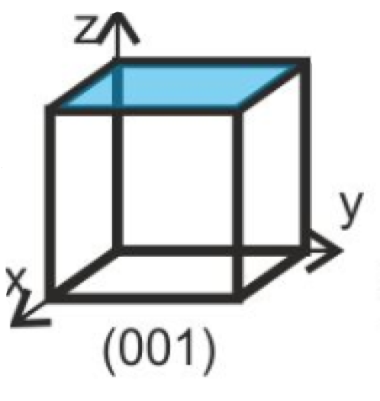
\includegraphics[scale = 0.4]{001.png}
            \caption{Stellt die (001)-Ebene graphisch dar.[1]}
            \label{A1}
        \end{minipage}
        \hfill
        \begin{minipage}[t]{0.45\linewidth}
            \centering
            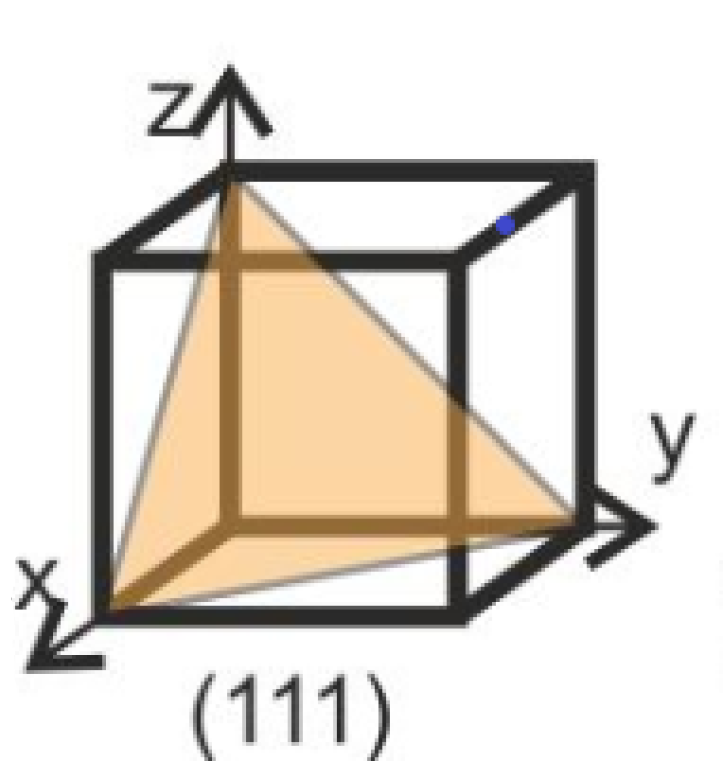
\includegraphics[scale = 0.25]{111.png}
            \caption{Stellt die (111)-Ebene graphisch dar.[1]}
            \label{A2}
        \end{minipage}
\end{figure}
Der (001) Reflex ist ein Überstruckturreflex und wächst bei zunehmender Ordnung, wohingegen der (111) Reflex ein Fundamentalreflex ist und sich mit längerer Wartedauer am Phasenübergang nicht ändert. Das Ziel dieses Teil des Berichtes ist herauszufinden, wie sich der Ordnungsparameter ändert. Dazu wird der Ordnungsparameter $\eta$ ,gemäß des JMAK-Modells[2], eingeführt. \\
\begin{align}
    \eta^2 &= {\frac{I_\text{exp}^{Ü}}{I_\text{exp}^{F}}}
    \cdot 
    ({\frac{(f_\text{Au}+3f_\text{Cu})^{F}}{(f_\text{Au}-f_\text{Cu})^{Ü}}})^{2}
    \cdot
    {\frac{p^{F}}{p^{Ü}}}
    \cdot
    {\frac{L_\text{p}^{F}}{L_\text{p}^{Ü}}}
    \cdot
    {\frac{D_\text{T}^{F}}{D_\text{T}^{Ü}}}
    \label{F1}
\end{align}
 Dabei sind die einzelnen Komponenten Wie folgt definiert. Die Buchtaben "Ü" und "F" stehen dabei für die jeweiligen Faktoren der Überstrukturreflexe bzw. der Fundamentalstrukturreflexe. Die Intensität des Überstrukturreflexes ist $I_\text{exp}^{Ü}$ und die Intensität des Fundamentalreflexes ist $I_\text{exp}^{F}$. Diese werden aus den Messungen abgelesen.
 Die Atomformfaktoren sind $f_\text{Au}$ und $f_\text{Cu}$. Diese sind für die Überstrukturreflexe und den Fundamentalreflexen identisch. Diese berücksichtigen die Lage der Atome in einer Elementarzelle. Um die Formfaktoren zu berechnen benötigt man Parameter $a_i$,$b_i$ und $c$. Diese werden aus [2] entnommen.
 Der Flächenhäufungsfaktor $p$ berücksichtigen wie häufig die einzelnen Netzebenen vorkommen. 
 Der Lorentz-Polarisationsfaktor $L_\text{p}$ werden geometrische Effekte der Röntenstrahlung korrigiert.
 Mit dem Debye- Waller-Faktor $D_\text{T}$ wird der Einfluss der Wärmebewegung mitberücksichtigt. Hierfür muss eine Konstante (B) ermittelt werden, die für 400°C $B = 1,6187$ ist.
 Die jeweiligen Faktoren wurden, wie in [2] angegeben berechnet. 
 \begin{align}
     f_\text{Atom} &= \sum_{i=0}^N a_i\exp{(-b_is^2)} +c
 \end{align}
 \begin{align}
     p_\text{(001)} &= 6 \\
     p_\text{(001)} &= 8
 \end{align}
\begin{align}
    L_\text{p} = \frac{1+\cos{2\theta}^2}{\sin{\theta}^2\cdot\cos{\theta}}
\end{align}
\begin{align}
    D_\text{T} &= \exp{(-2B\frac{\sin{\theta}^2}{\lambda^2})} \\
    B &= 1,6187
\end{align}
Als letzten Aspekt wurde der Fernordnungsparameter auf die Zeit aufgetragen um zu beschreiben, wie sich die Dynamik von $\eta$ verhält. Nach dem JMAK-Modell soll die zeitliche Veränderung beschrieben werden durch eine Konstante (k), die von der Nukleationsrate und der Wachstumsgeschwindigkeit der Keime abhängig ist und dem Avrami-Exponenten (n).
\begin{align}
    \eta(t) = 1- exp(-kt^n)
\end{align}
Dabei wird überprüft, ob der theoretische Wert von $\eta = 4$ angenommen wird.

\section{Auswertung}
Als erstes wird die Dynamik des (001) Überstrukturreflex analysiert. Die erste und die zweite Messung sind vom Rauschen überzogen, sodass nicht erkannt werden kann ob überhaupt ein Reflex auftaucht. Mit der Zeit bildet sich ein Peak aus, welches sich vom Rauschen abhebt. Ab der 15. Messung ist zu sehen, dass sich ein Überstrukturreflex gebildet hat.
\begin{figure}[h!]
    \centering
    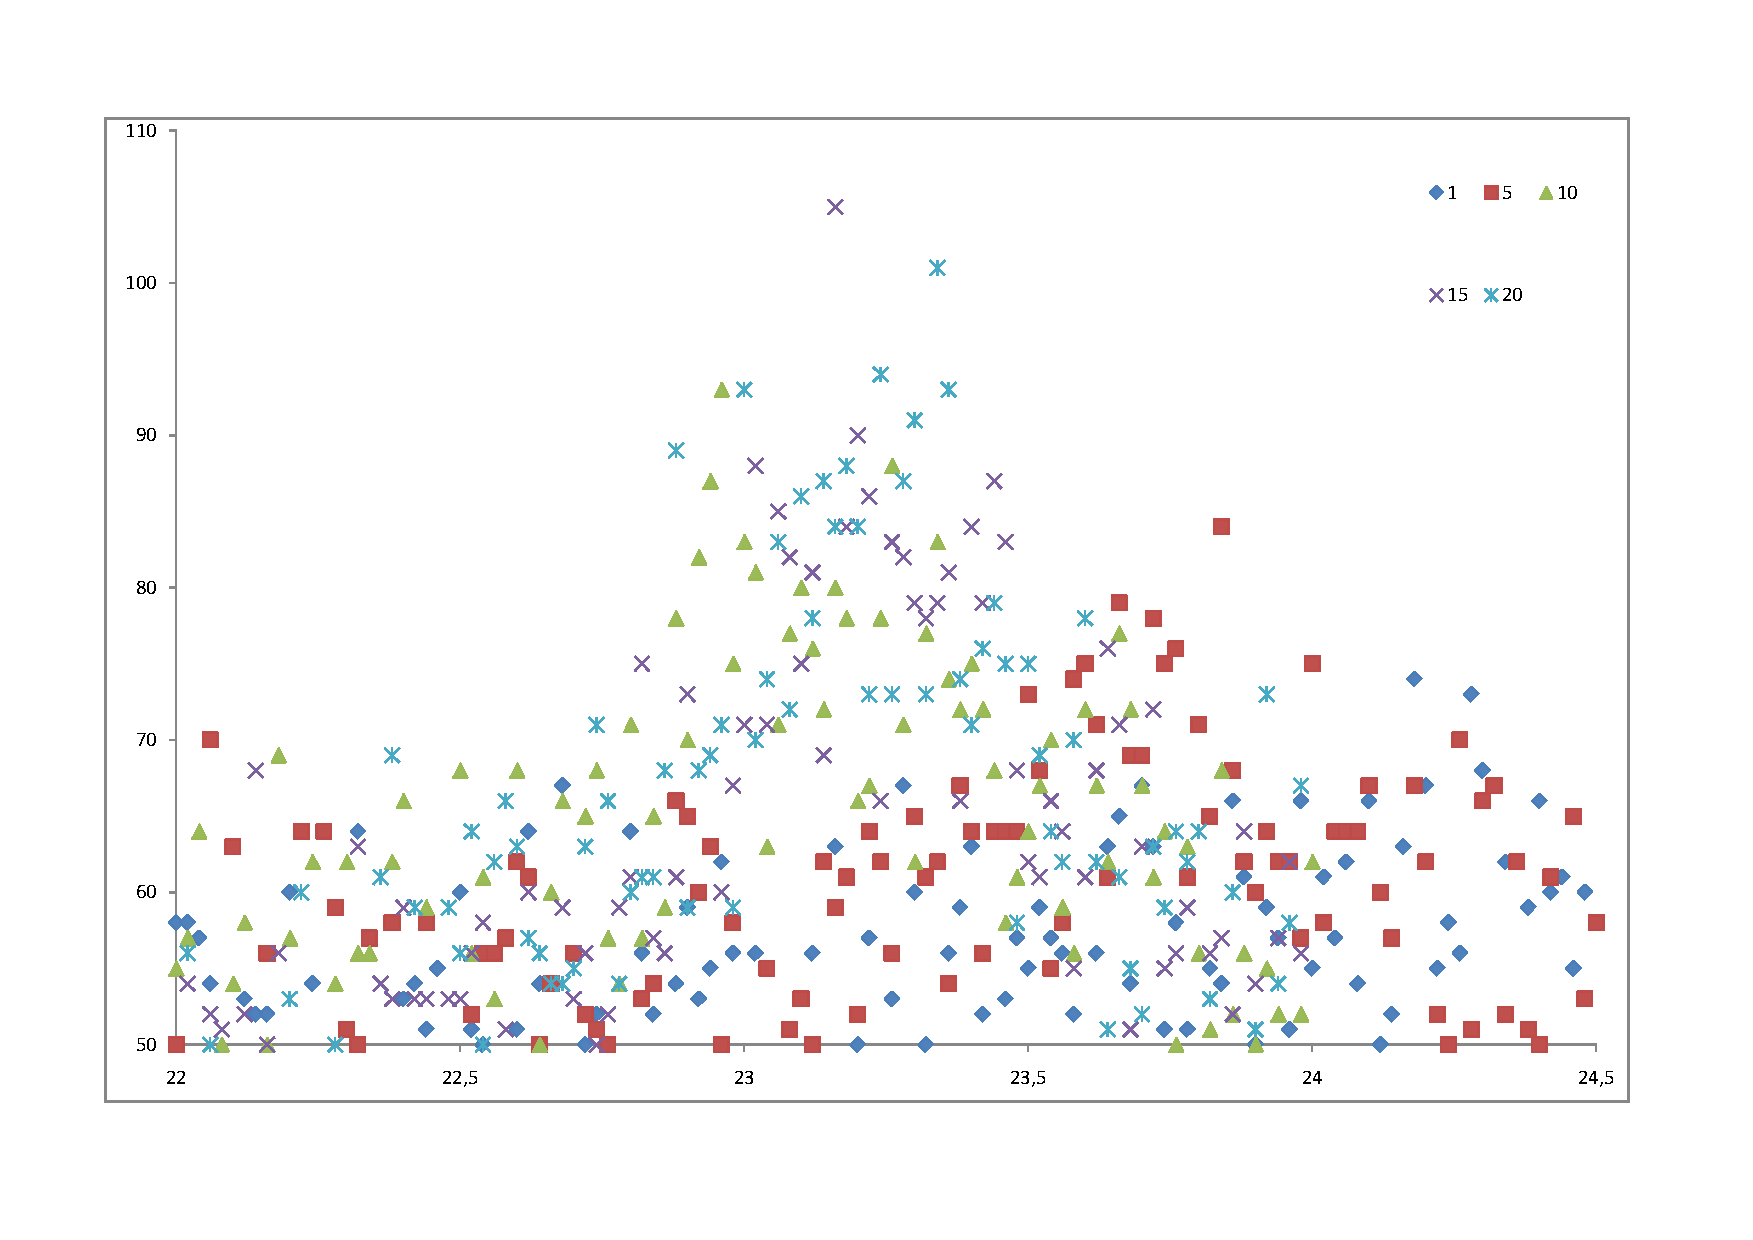
\includegraphics[scale = 0.6]{Bragg.pdf}
    \caption{Diese Graphik stellt die Dynamik (001)-Ebene dar. Auf der $x$-Achse ist der Winkel in Grad angegeben und auf der $y$-Achse ist die Intensität angegeben der einfallenden Röntenstrahlung. Die dunkel blauen Rauten sind die ersten Messungen. Die roten Quadrate die fünften Messungen die grünen Dreiecke sind die zehnten Messungen die violetten Kreuze die 15. Messungen und die hell blauen Kreuze sind die 20. Messung.}
    \label{A3}
\end{figure}
Anhand von \cref{A3} konnte beobachtet werden, dass sich innerhalb der Messwerte nach der 15. Messung nicht mehr viel in der Dynamik abgespielt hat, sodass dies als neue Phase erkannt wurde. Durch diesen stationären Zustand kann der Ordnungsgrad ermittelt werden. Dieser lag bei kleinen Temperaturen (25°C) bei $\eta = 1$ und bei hohen Temperaturen(x > 700°C) bei $\eta = 0$. Da ein Maß der Ordnung $\eta$ darstellt und dies gerade das Verhältnis von dem (001) und (111) Reflex nach \cref{F1} ist, werden deren Größenordungen, bei 400°C durch \cref{A3} veranschaulicht.
\begin{figure}[h!]
    \centering
    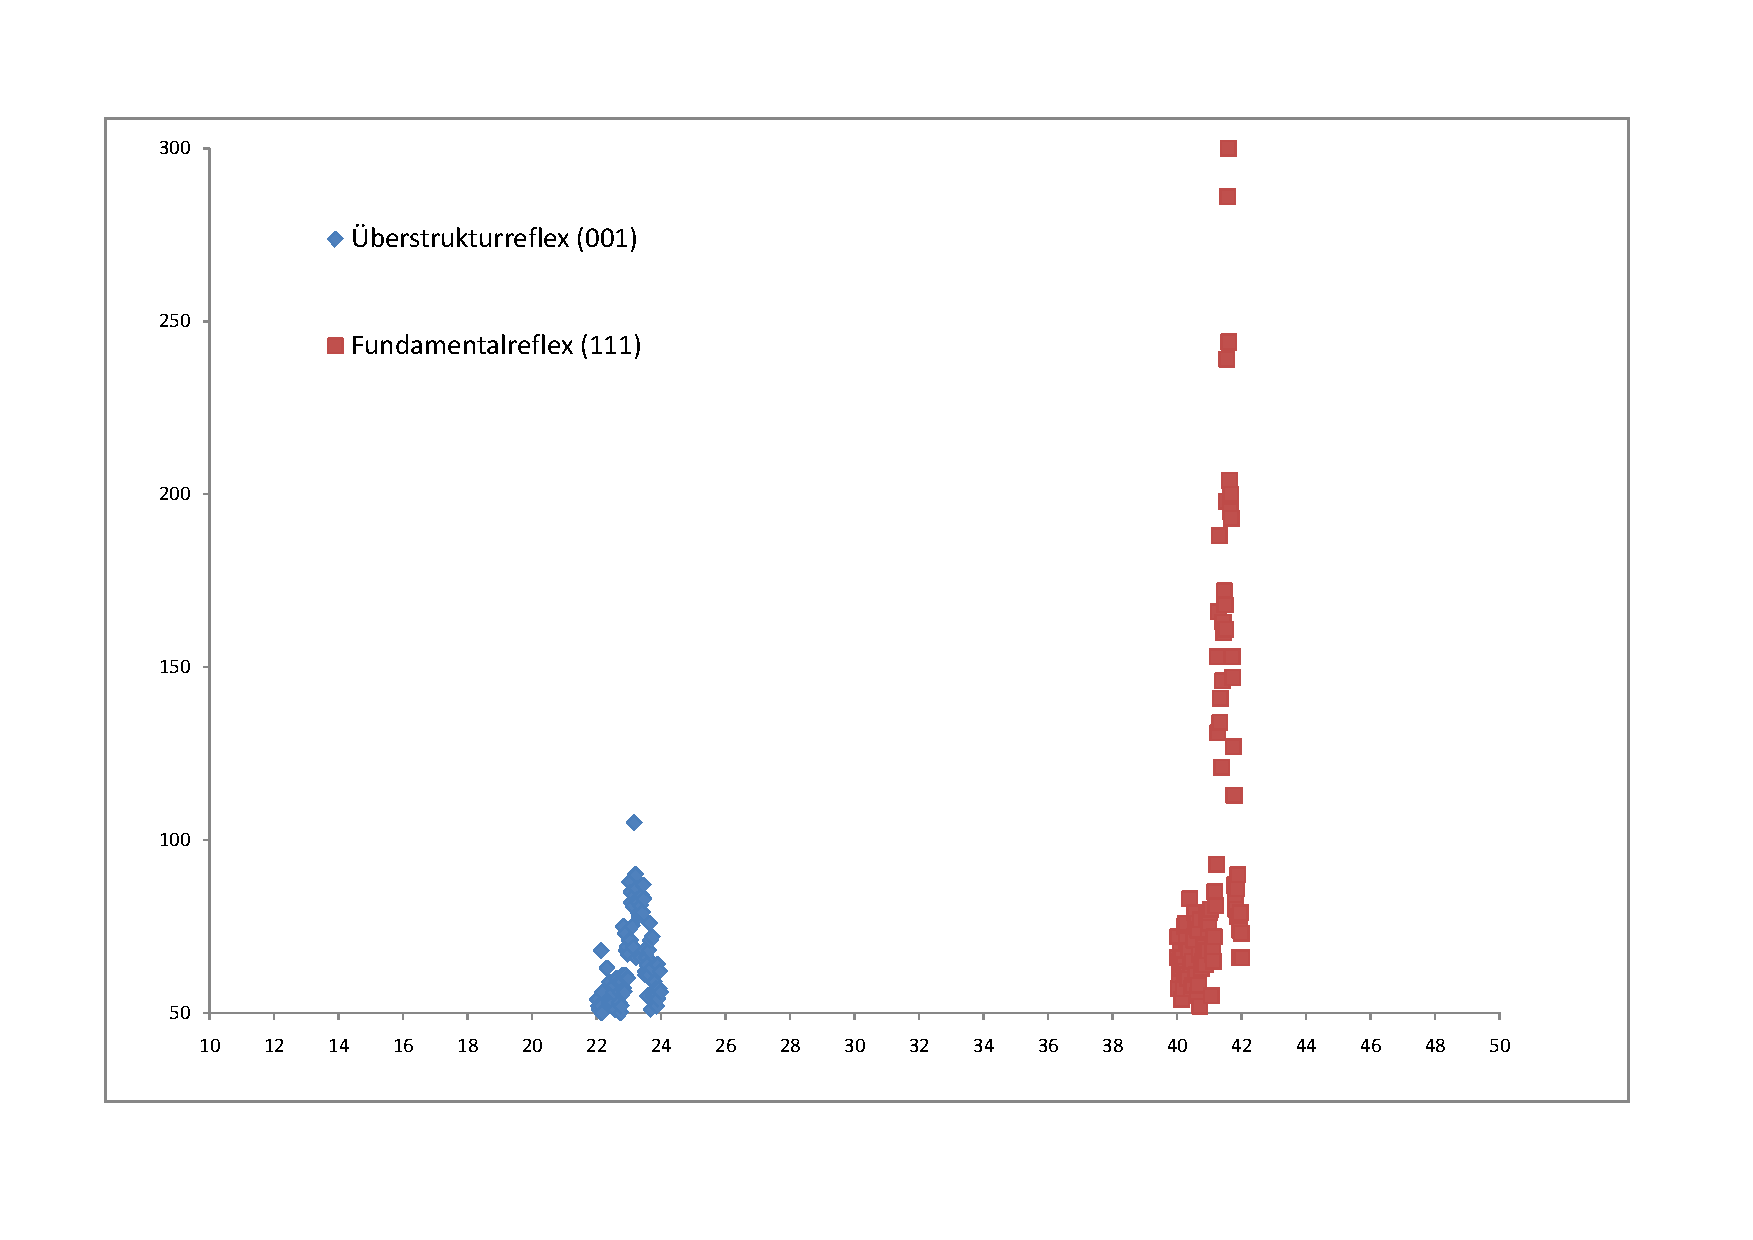
\includegraphics[scale = 0.6]{001 und 111.pdf}
    \caption{Diese Graphik stellt die (001) und die (111) Reflexe im stationären Zustand dar. Auf der $x$-Achse ist der Winkel in Grad angegeben und auf der $y$-Achse ist die Intensität angegeben der einfallenden Röntenstrahlung. Der Überstrukturreflex stellt die 15. Messung dar. Wohingegen der Fundamentalreflex sich über die Zeit nicht geändert hat.}
    \label{A4}
\end{figure}
Der Überstrukturreflex ist die 15. Messung die gemacht wurde. Diese Messung wurde zur bildlichen Darstellung benutzt, da diese den höchsten Wert innerhalb der Messreihe besessen hat. Während der Auswertung wurde jedoch mit allen Messwerten gerechnet.
Über Formel \cref{F1} wurden die Ordnungsparameter bestimmt. Dazu wurde bei dem (111) Reflex ein Mittelwert der beiden Referenzwerte genommen, um näher beim statistischen Mittel zu liegen. Der (111) Wert hat sich mit der Zeit kaum geändert, sodass hier ein, mit den variierenden Parametern, zeitlicher konstanter Peak angenommen wurde. Um ein Mittel bzgl. dieser beiden Messwerte zu benutzen wurde der Mittelwert betrachtet. In \cref{A4} können die Messpunkte betrachtet werden. 
\begin{figure}[h!]
    \centering
    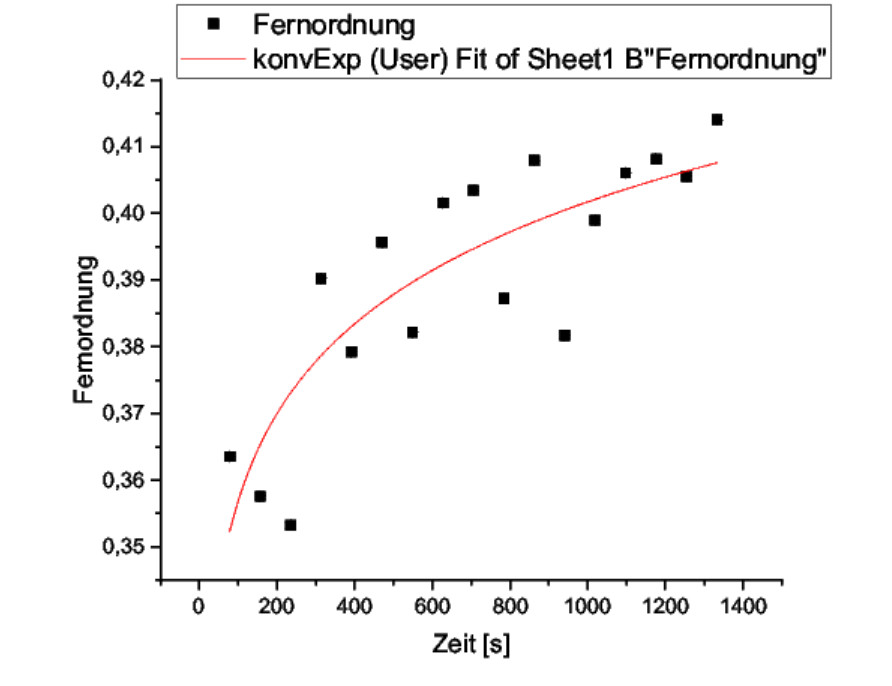
\includegraphics[scale = 0.7]{M3/tex/fit.png}
    \caption{Die Ordnung steigt mit zunehmender Zeit. Vor dem Anstiegt hatte die Ordnung einen festen Wert. Nach dem Anstieg wird der Wert  ebenfalls auf einem Wert verharren bis sich die Phase wieder ändert. Sodass hier ein logistisches Wachstum der Ordnung angenommen werden kann.Hier ist nur der Ausschnitt des Wachstums dargestellt. Der Fit besitzt folgende Form. Die Messunsicherheiten sind dabei so klein, dass diese nicht zu sehen sind. Der Fit wurde mit OriginPro berechnet.
    $\eta = 1 - exp(-kt^n)$ mit $k=0,32 \pm 0,02$ und $n=0,07 \pm 0,01$}
    \label{A5}
\end{figure}

Nun wurden die Ordnungsparameter berechnet und auf \cref{A5} dargestellt. Die Zeitbalken auf der $x$-Achse müssen nicht immer denselben Abstand haben. Diese Unsicherheit wurde im folgenden ignoriert. Dieser Graph zeigt wie sich die Ordnung beim Phasenübergang verhält. Vor dem Phasenübergang existierte eine Stabile Ordnung. Dann wird die Ordnung bei der Phasenumwandlung so lange verändert bis eine neue Ordnung entsteht die wieder stabil ist. In \cref{A5} ist jedoch nur die Dynamik des Übergangs dargestellt. Anhand des Fits können folgende Parameter bestimmt werden. \\
$\eta = 1 - exp(-kt^n)$ mit $k=0,32 \pm 0,02$ und $n=0,07 \pm 0,01$\\
Hieraus kann abgelesen werden, dass der Avrami-Exponenten nicht den theoretischen Wert von n=4 angenommen hat.


\section{Unsicherheit}
Um die Unsicherheiten zu berechnen wurde geschaut, welche Messungen die höchste Messunsicherheit hatte. Innerhalb unserer Messwerte konnte die größte Messunsicherheit der Intensitätsmessung zugewiesen werden, sodass diese durch eine Dreickswahrscheinlichkeitsdichtefunktion abgeschätzt wurde. Alle anderen Messwerte wurden vernachlässigt, da diese zur Gesamtunsicherheit vernachlässigar sind.
\begin{align*}
    u_{I_\text{max}} &= \frac{1[I]}{2\sqrt{6}} &= 0,02[I]
\end{align*}
Die weiteren Rechnungen wurden dann mithilfe der Fehlerfortpflanzung ermittelt. Diese wurde nur bei den Termen angewandt, wo der größte Fehler aufgetreten ist.
\begin{align*}
    u_{\eta^2}^2 &= ({\frac{1}{I_\text{exp}^{F}}}
    \cdot 
    ({\frac{(f_\text{Au}+3f_\text{Cu})^{F}}{(f_\text{Au}-f_\text{Cu})^{Ü}}})^{2}
    \cdot
    {\frac{p^{F}}{p^{Ü}}}
    \cdot
    {\frac{L_\text{p}^{F}}{L_\text{p}^{Ü}}}
    \cdot
    {\frac{D_\text{T}^{F}}{D_\text{T}^{Ü}}}u_{I_\text{max}^{Ü}})^2 + 
    ({\frac{I_\text{exp}^{Ü}}{I_\text{exp}^{F}^2}}
    \cdot 
    ({\frac{(f_\text{Au}+3f_\text{Cu})^{F}}{(f_\text{Au}-f_\text{Cu})^{Ü}}})^{2}
    \cdot
    {\frac{p^{F}}{p^{Ü}}}
    \cdot
    {\frac{L_\text{p}^{F}}{L_\text{p}^{Ü}}}
    \cdot
    {\frac{D_\text{T}^{F}}{D_\text{T}^{Ü}}}u_{I_\text{max}^{F}})^2
\end{align*}
Weitere Unsicherheiten wurden über den Fit bestimmt, der mit OriginPro berechnet wurde.


\section{Diskussion}
Innerhalb dieser Auswertung wurde eine Näherung für die Dynamik bei einem Phasenübergang gemacht. Da der (001) Reflex wieder auftaucht kann darauf geschlossen werden, dass die Ordnung im Kristall zunimmt, da neue Symmetrien auftauchen. Anhand von \cref{A5} kann gesehen werden, dass die Ordnung zwischen (0,4-0,6) liegt. Dies entspricht unseren Erwartungen, da Null vollständige Unordnung entsprach, wohingegen 1 der vollständigen Ordnung entsprach. Da die Temperatur inmitten der zugeordneten Temperaturskala (25°C - 700°C) liegt, ist es logisch, dass auch der Ordnungsparameter in etwa in der Mitte der Werte liegt. Das ein Anstieg zu begutachten ist ist auch plausibel, da einmal der Phasenübergang eine zeitliche Entwicklung braucht, aber auch weil von 400°C auf 375°C reduziert wurde. So könnte ein zeitlich Veränderliches B (Debye-Waller-Faktor) zur genaueren Untersuchung dieses Sachverhaltes eingebaut werden. Der berechnete Fit stimmt jedoch zu der theoretischen Überlegung von n=4 nicht. In diesem Fall wurde n zu $n=0,07 \pm 0,01$ berechnet. Um diesen Sachverhalt genauer zu beleuchtet, wird erstmal erklärt, wieso der Exponent n=4  herausgefunden werden sollte. Zum einen steigt die Anzahl der Keime (N) gemäß $N \cdot t$ an und jeder einzelne Keim wächst in jeder Dimension mit $t$, folglich $t^3$. Es könnte an dem Versuchsaufbau liegen, dass nicht n=4 herausgekommen ist, da nur an der Oberfläche gemessen wurde und so die Keimausbreitung nur noch mit $t^2$ steigt, sodass ein Wert zwischen 3-4 erwartet werden würde. Dies erklärt dennoch immer noch nicht den Wert von $n=0,07 \pm 0,01$, sodass der Fehler im Fit liegen muss. Es könnte sein, dass das Programm zu wenig variable Parameter besessen hatte um die Messwerte gut genug abzubilden. So müsste ein Verschub in der Zeit, eine andere Amplitude oder ein Offset der Daten berücksichtigt werden, um näher am theoretischen Ergebnis zu landen. So ist die Gleichung vom JMAK-Modell nicht an Experimentelle Messdaten angepasst, sodass an der zu fittenden Funktion eine Änderung vorgenommen werden müsste.

\section{Literaturverzeichnis}
[1] \url{https://www.researchgate.net/figure/Miller-indices-indicating-the-plane-perpendicular-to-the-vector-given-for-the-cubic_fig7_302838100}\\
[2] Charakterisierung der Phasenumwandlung in Kupfer-Gold Legierungen,Fortgeschrittenen Praktikum, Versuchsanleitung, Münster ,WS 18/19










% --- Anhang einbinden
\IfFileExists{tex/20_Anhang.tex}{
	\clearpage
	\appendix
	\section{Anhang}
	\label{sec:anhang}
	\input{tex/20_Anhang.tex}
}{}

% --- Literaturverzeichnis mit BibLaTeX
\ifthenelse{\boolean{showBibliography}}{
	\clearpage
	\printbibliography
}{}

\end{document}

